\documentclass[letterpaper,12pt]{article} %tipo de documento y tama~o de papel y letra
\usepackage[latin1]{inputenc} %codificacion de caracteres
\usepackage[spanish]{babel} %idioma
\usepackage{fancyhdr} %tipo de pagina, LINDA biggrin.gif
\usepackage[top=3.5cm,bottom=2.5cm,right=2cm,left=2.5cm]{geometry} %margenes
\usepackage[rflt]{floatflt} %ni puta idea
\usepackage{pdfpages} %incluir archivos pdf
\usepackage{hyperref} %hipervinculos
\hypersetup{
  colorlinks=true,
  urlcolor=cyan
}
%\usepackage{helvet} %esto es pa escribir con Arial en vez de times new roman
%\renewcommand\familydefault{\sfdefault} %descomenta estas lineas para escribir en arial

\usepackage{multirow}

\usepackage{graphicx} %para usar imagenes
%\newcommand{\imgdir}{doc-img} % para meter las imagenes en una carpeta especial, tunz en la carpeta del documento tiene q ir otra que se llame 'doc-img'
\graphicspath{{./pic/}} %le dice que las imagenes estan en la carpeta de arriba

\usepackage{amsmath} %pa usar smbolos matematicos
\numberwithin{equation}{section} % pa usar ecuaciones de modo lindo
\numberwithin{figure}{section} %para agregar imagenes
\numberwithin{table}{section} %para agregar tablas

\usepackage{subfigure} % pa usar sub figuras



\pagestyle{fancy} %configuracion para la pagina linda
\renewcommand{\sectionmark}[1]{\markboth{}{\thesection\ \ #1}} %cambios de comentarios
\lhead{} %parte de arriba, izq
\chead{} %parte de arriba, centro
\rhead{\rightmark} %parte de arriba, derecha, le agrega la marca del capitulo
\lfoot{} %parte de abajo, izq
\cfoot{} %parte de abajo, centro
\rfoot{\thepage} %parte de abajo, derecha, va el numero de la pagina


%-------------portada---------------------------------%
\begin{document}
\begin{titlepage} %portada
\thispagestyle{empty} %borrar el formato de pagina linda
%\begin{flushleft} %alinear a la izq
\begin{center}

\includegraphics[scale=0.35]{logoUSM-DI.eps}
%\vfill
\end{center}
%\end{flushleft}

\vspace{3cm} %espacio vertical , en realidad es un enter de 2 cm
\begin{center} %centrar
{\Huge Requerimientos de Software \\
 \huge Proyecto ``\emph{V.I.Pe.R.}''\\
  \normalsize\today
}
\end{center}

\vspace{6cm}

\vfill
\begin{flushleft} %alinear derecha
Pre-Empresa: \emph{Phyrex}\\
Jefe de Proyecto: Rodrigo Fr\'{\i}as\\
Integrantes:
\begin{table}[hb]
  \begin{tabular}{lcc}
    Rodrigo Fr\'{\i}as & \texttt{\small <rodrigo.frias@alumnos.usm.cl>} & [+56 9 83988257] \\
    Celeste Bertin & \texttt{\small <celeste.bertin@alumnos.usm.cl>} &[+56 9 68410901]\\
    Patricio Carrasco &\texttt{\small <patricio.carrascod@alumnos.usm.cl>} &[+56 9 50626689]\\
    Rocio Fernandez &\texttt{\small <rocio.fernandezu@alumnos.usm.cl>} & [+56 9 62426549]\\
    Juan Avalo & \texttt{\small <juan.avalo@alumnos.usm.cl>} & [+56 9 78072458]\\
  \end{tabular}
\end{table}
\end{flushleft}
\end{titlepage}
%------------------fin de la portada --------------------%

%{\bf } %escribir en negrita

\setcounter{page}{1} %empezar enumerando la pagina 1

\tableofcontents
\newpage

\section{Ficha de Clasificaci\'on R\'apida}
\subsection{Objetivo del Proyecto} %140 caracteres
\subsection{Resumen del Proyecto} %media pagina
\subsection{Cliente}
Nombre: Jocelyn Simmonds\\
Cargo: \\
E-mail: jsimmond@inf.utfsm.cl\\
Tel\'efono: \\
Rol o Experiencia relevante al producto:

\newpage
\section{Modelo de Dominio}

\begin{figure}
   \centering
     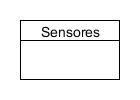
\includegraphics[scale=0.5]{ModeloDominio.jpg}
   \caption{Se puede apreciar el Modelo de Dominio relativo a \emph{V.I.Pe.R}.}
   \label{fig:ModeloDominio}
\end{figure}


\begin{table}[hb!]
  \begin{tabular}{lp{7cm}}\hline
    Entidad & Descripci\'on \\ \hline \hline %1 linea
    & \\ \hline
  \end{tabular}
\end{table}

\newpage
\section{Actores y Tareas Clave}

\begin{table}[hb!]
  \begin{tabular}{lp{7cm}}\hline
    Actor & Descripci\'on \\ \hline \hline %1 linea
    & \\ \hline    
  \end{tabular}
\end{table}

\begin{table}[hb!]
  \begin{tabular}{lp{7cm}}\hline
    Tarea Clave & Descripci\'on \\ \hline\hline %max 3 lineas
    & \\ \hline
  \end{tabular}
\end{table}

\newpage
\section{Requerimientos Extra-funcionales}

\begin{table}[hb!]
  \begin{tabular}{lp{7cm}}\hline 
    Req. Extra-funcional & Descripci\'on y medici\'on \\ \hline\hline %max 2 lineas
    & \\ \hline
  \end{tabular}
\end{table}

\newpage
\section{Restricciones de Software y Hardware}

A continuaci\'on se detallan las restricciones propias del Software y del Hardware, tanto en las limitantes de comunicaci\'on entre ellos, como en lo solicitado por el cliente.

\begin{table}[hb!]
  \begin{tabular}{p{3cm}p{7cm}}\hline
    Restricci\'on & Raz\'on \\ \hline\hline %max 2 lineas
    Sistema rob\'otico debe ser LEGO Mindstorm NXT & Herramienta para principiantes, permite mayor manipulaci\'on y dinamicidad a la construcci\'on, adem\'as de ser atractivo para el usuario.\\ \hline
    Aplicaci\'on m\'ovil debe programarse para smartphones con OS Android & Facilidad en la disponibilidad del recurso de trabajo. \\ \hline
    Conectividad entre mascota f\'isica y aplicaci\'on debe ser por bluetooth & Resulta de las restricciones anteriores. Es la tecnolog\'{\i}a que tienen en com\'un para comunicarse entre ellos.\\ \hline \hline
  \end{tabular}
\end{table}

\newpage
\section{Casos de Uso} %al menos 3 casos de uso no-triviales

En la figura~\ref{fig:CasoUso}, se puede apreciar los casos de uso del proyecto, englobando algunos en un nivel de abstracci\'on alto.

\begin{figure}[h!]
   \centering
     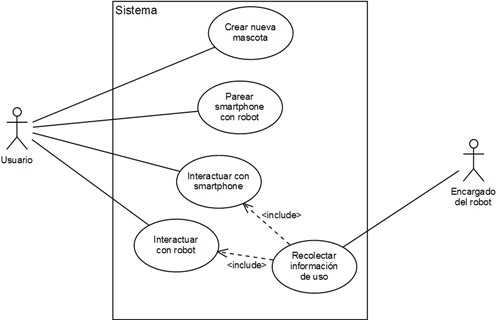
\includegraphics[scale=0.5]{CasoUso.jpg}
   \caption{Es posible apreciar algunos Casos de Uso relativos al proyecto \emph{V.I.Pe.R.}.}
   \label{fig:CasoUso}
\end{figure}

Respecto a los casos de uso no-triviales, cabe destacar tres que son necesarios para la aplicaci\'on, en distintos niveles de aplicaci\'on. Por un lado, est\'a el caso de uso ``Crear Mascota'' que hace referencia a la interacci\'on entre usuario y el smartphone con Android, y es el que se detalla en~\ref{tab:Crear}.

\begin{table}[hb!]
  \begin{tabular}{p{3cm}p{7cm}}\hline\hline
    Nombre: & Crear Mascota. \\ \hline
    Descripci\'on: & El usuario al utilizar la aplicaci\'on Android por primera vez, debe crear una mascota virtual, que va a ser el medio de interacci\'on entre dicho dispositivo y el robot Lego Mindstorms\\ \hline %max 5 lineas
    Pre-condiciones: & No debe existir una mascota anteriormente.\\ \hline
    Post-condiciones: & Mascota Virtual creada y esperando para interactuar con el usuario\\ \hline
    Requerimienos no Funcionales: & ---\\ \hline\hline %min 0 ; max 3
  \end{tabular}
  \label{tab:Crear}
\end{table}

Luego, el segundo caso de uso se denomina ``Parear y Calibrar'', el que es posible observar m\'as en detalle en~\ref{tab:Parear}, y abarca el nivel de interacci\'on entre el equipo smarthphone y el robot Lego Mindstorms.

\begin{table}[hb!]
  \begin{tabular}{p{3cm}p{7cm}}\hline\hline
    Nombre: & Parear y Calibrar. \\ \hline
    Descripci\'on: & Es necesario poder transmitir datos desde la aplicaci\'on Android hacia el robot y viceversa, para ello es necesario poder comunicar los equipos. Adem\'as, estos deben poder funcionar correctamente en el medio en el que se encuentran.\\ \hline %max 5 lineas
    Pre-condiciones: & Smartphone Android y Robot Lego Mindstorms no pareados (sin comunicaci\'on entre ellos).\\ \hline
    Post-condiciones: & Smartphone Android y Robot Lego Mindstorms pareados (con comunicaci\'on entre uno y otro) y con la funcionalidad correspondiente al medio en que se encuentre el robot (fuerza de los motores seg\'un terreno, sensibilidad de sensores, etc.)\\ \hline
    Requerimienos no Funcionales: &
    \begin{itemize}
    \item Disponer de al menos 3 niveles de fuerza en motores encargados de movimiento.
    \end{itemize}\\ \hline\hline %min 0 ; max 3
  \end{tabular}
  \label{tab:Parear}
\end{table}

Finalmente tenemos el caso de uso ``Recolectar informaci\'on de uso'', que hace referencia al \'ambito de interacci\'on del caso~\ref{tab:Parear}, pero para un posterior uso del ``Encargado del Robot''. Este se encuentra en~\ref{tab:Recolectar}.

\begin{table}[hb!]
  \begin{tabular}{p{3cm}p{7cm}}\hline\hline
    Nombre: & Recolectar informaci\'on de uso.\\ \hline
    Descripci\'on: & Debido al objetivo en cuanto a difusi\'on, se hace necesario saber que tipo de futuros alumnos est\'an utilizando el sistema, y que tipo de uso se le da al mismo.\\ \hline %max 5 lineas
    Pre-condiciones: & ``Parear y Calibrar'', Usuario interactuando con el sistema.\\ \hline
    Post-condiciones: & Datos de uso de las funcionalidades de la aplicaci\'on.\\ \hline
    Requerimienos no Funcionales: & ---\\ \hline\hline %min 0 ; max 3
  \end{tabular}
  \label{tab:Recolectar}
\end{table}



%\newpage
%\chapter*{Anexo I - Presentaci\'on} %Copia Presentacion
%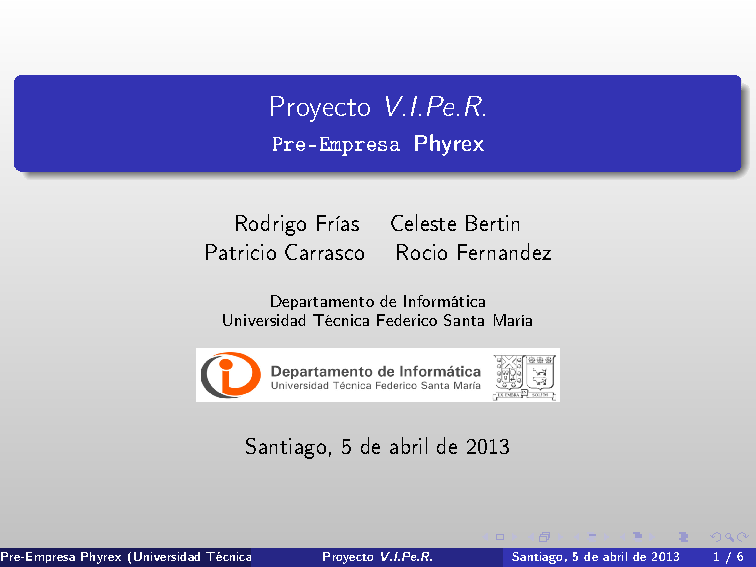
\includepdf[pages={1-},frame=true,nup=2x3,delta=10 20,scale=0.85]{../Presentacion/diapo-1x1.pdf}
%\newpage
%\chapter*{Anexo II - Curr\'{\i}culum Vitae} %Curriculum
%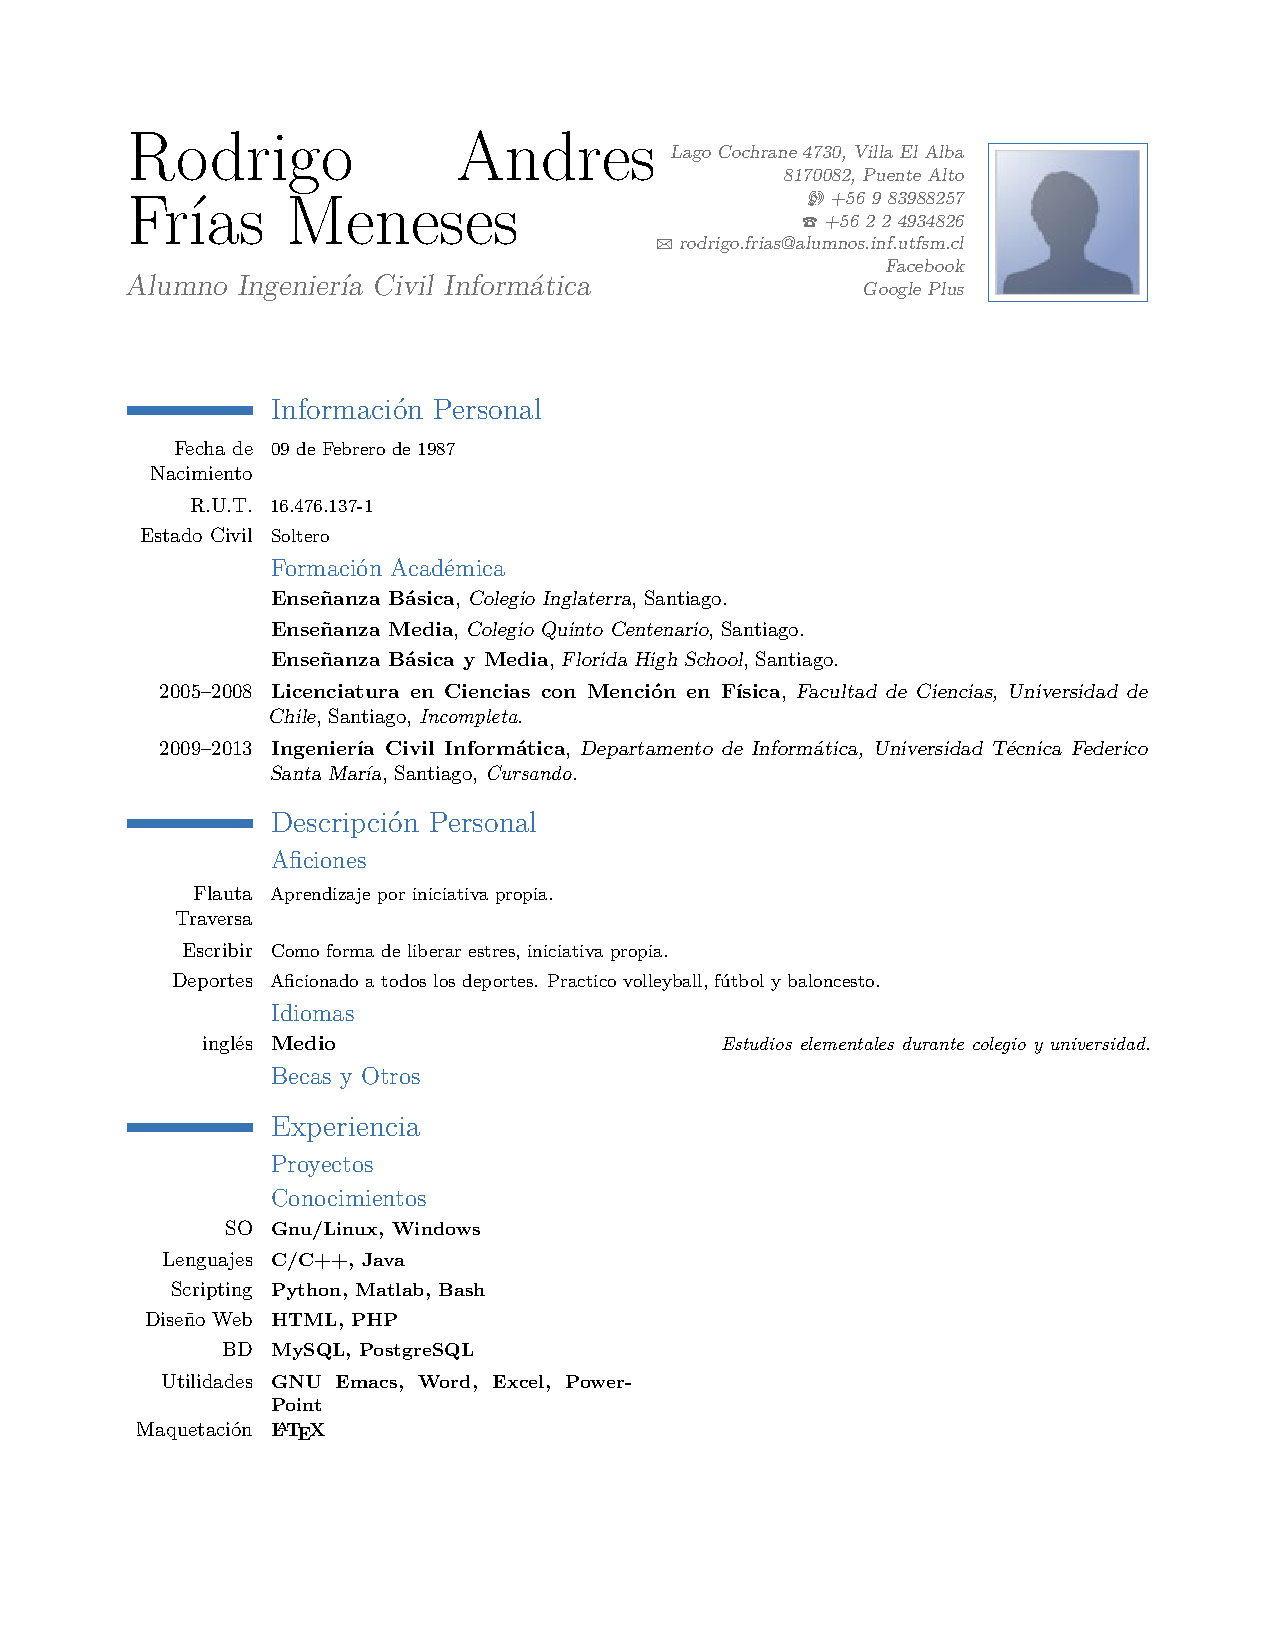
\includepdf[pages={1}]{../CV/cv-igo.pdf}
%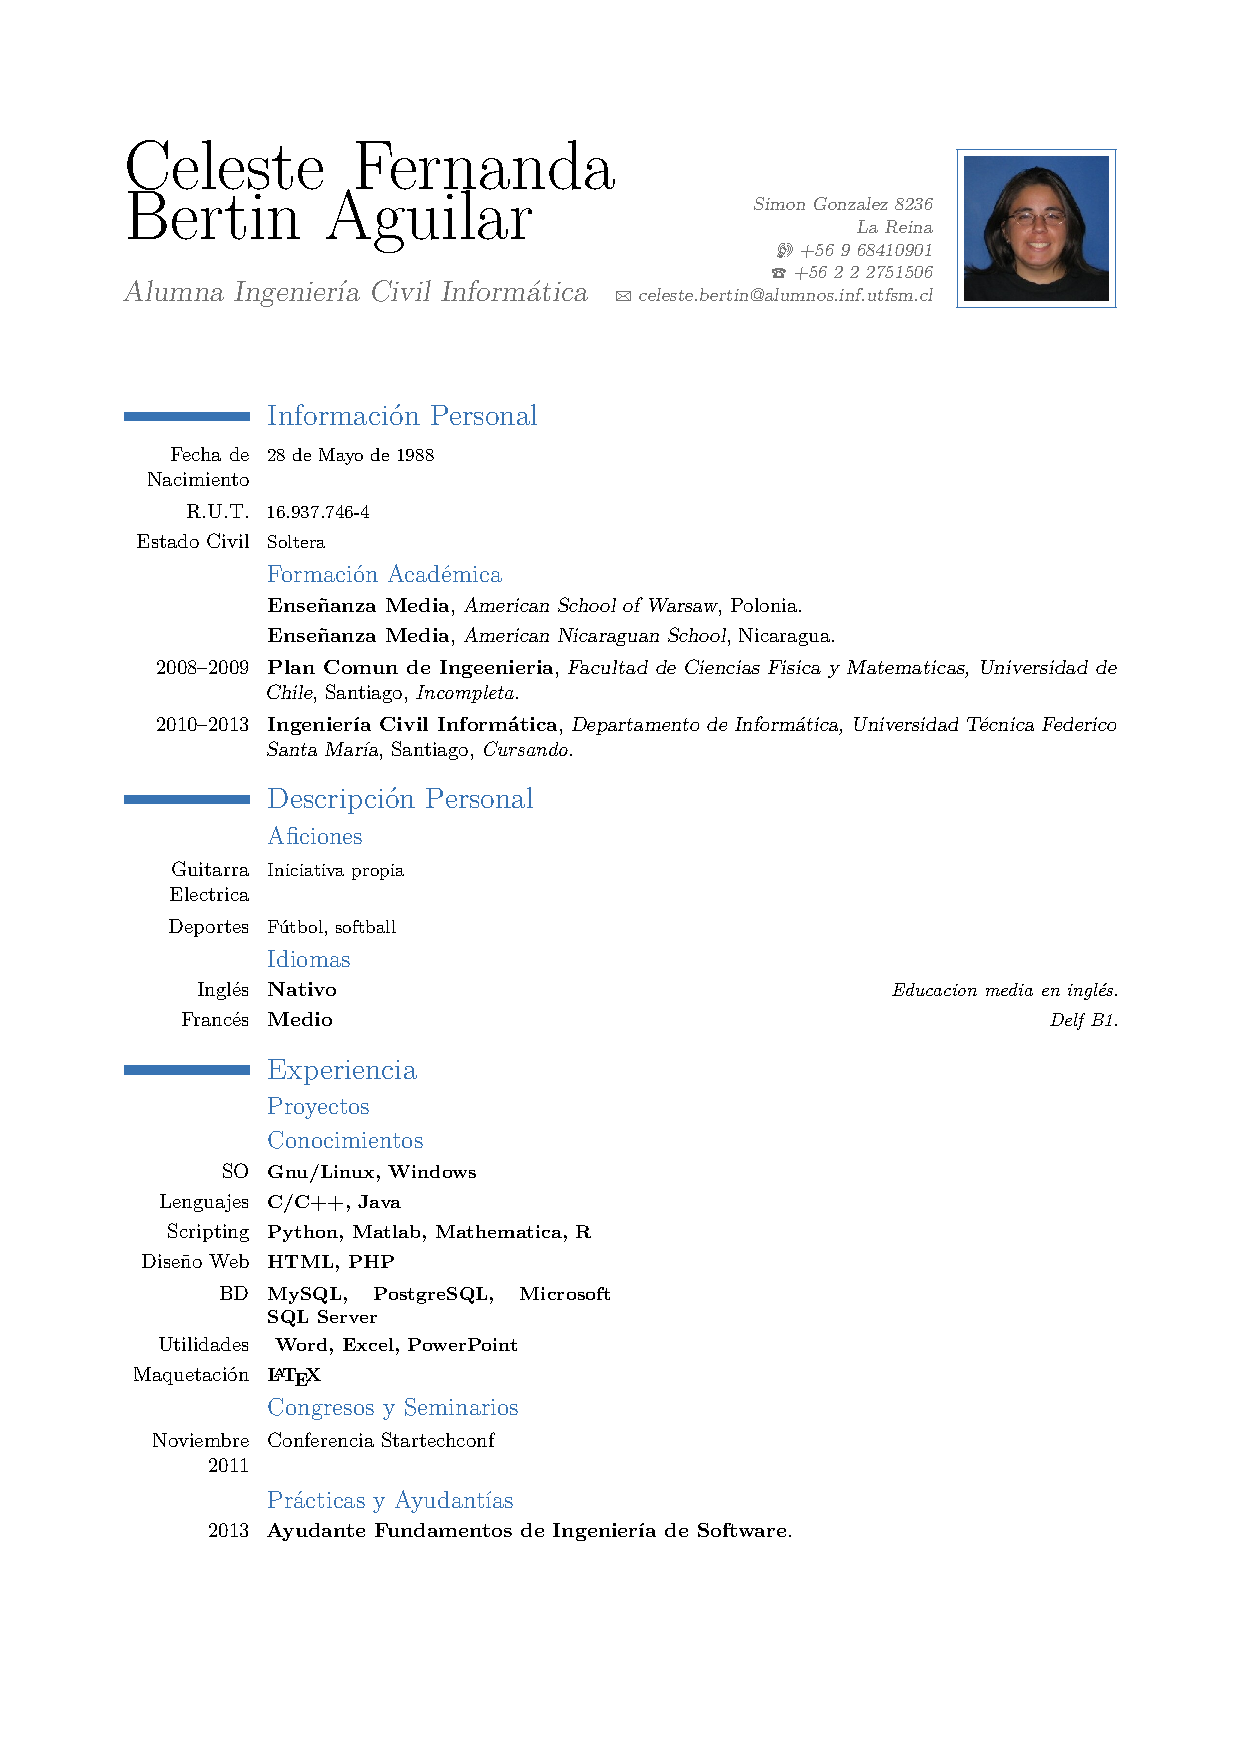
\includepdf[pages={1}]{../CV/cv-celeste.pdf}
%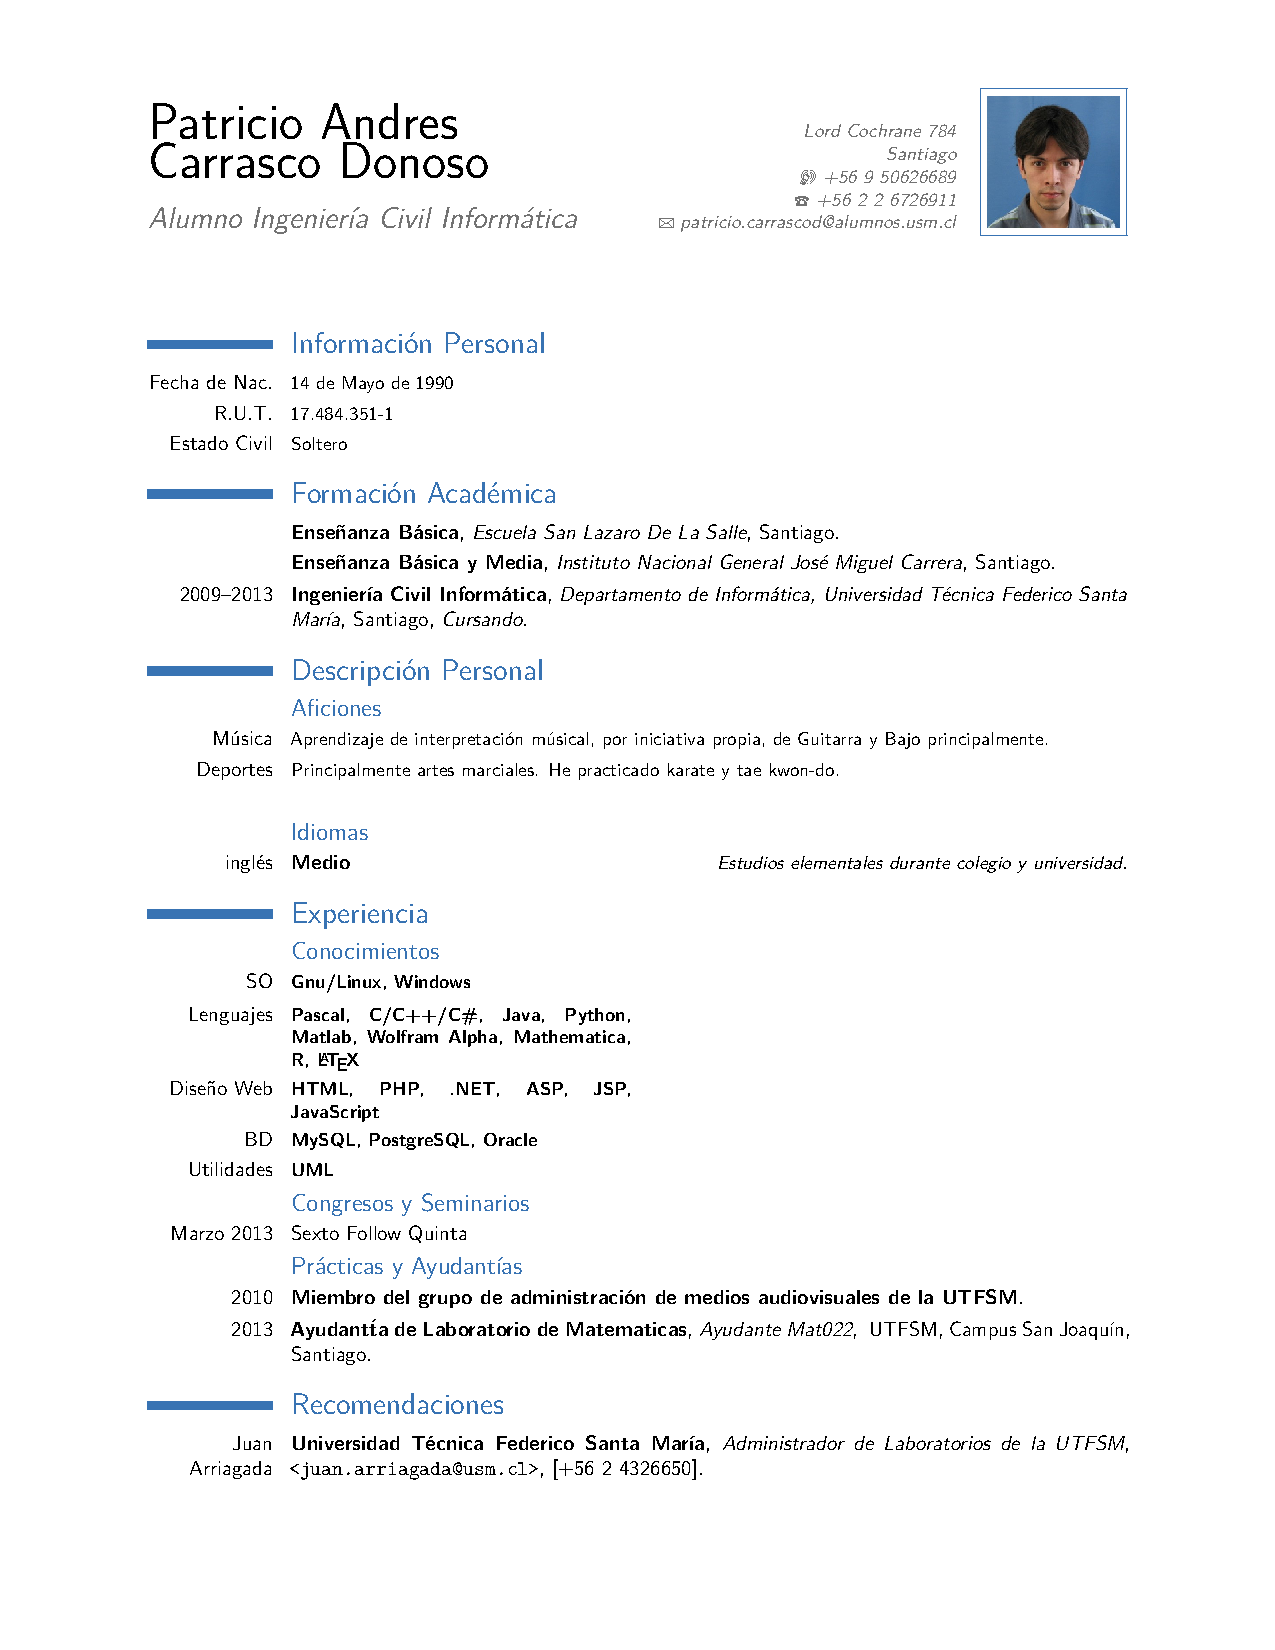
\includepdf[pages={1}]{../CV/cv-pato.pdf}
%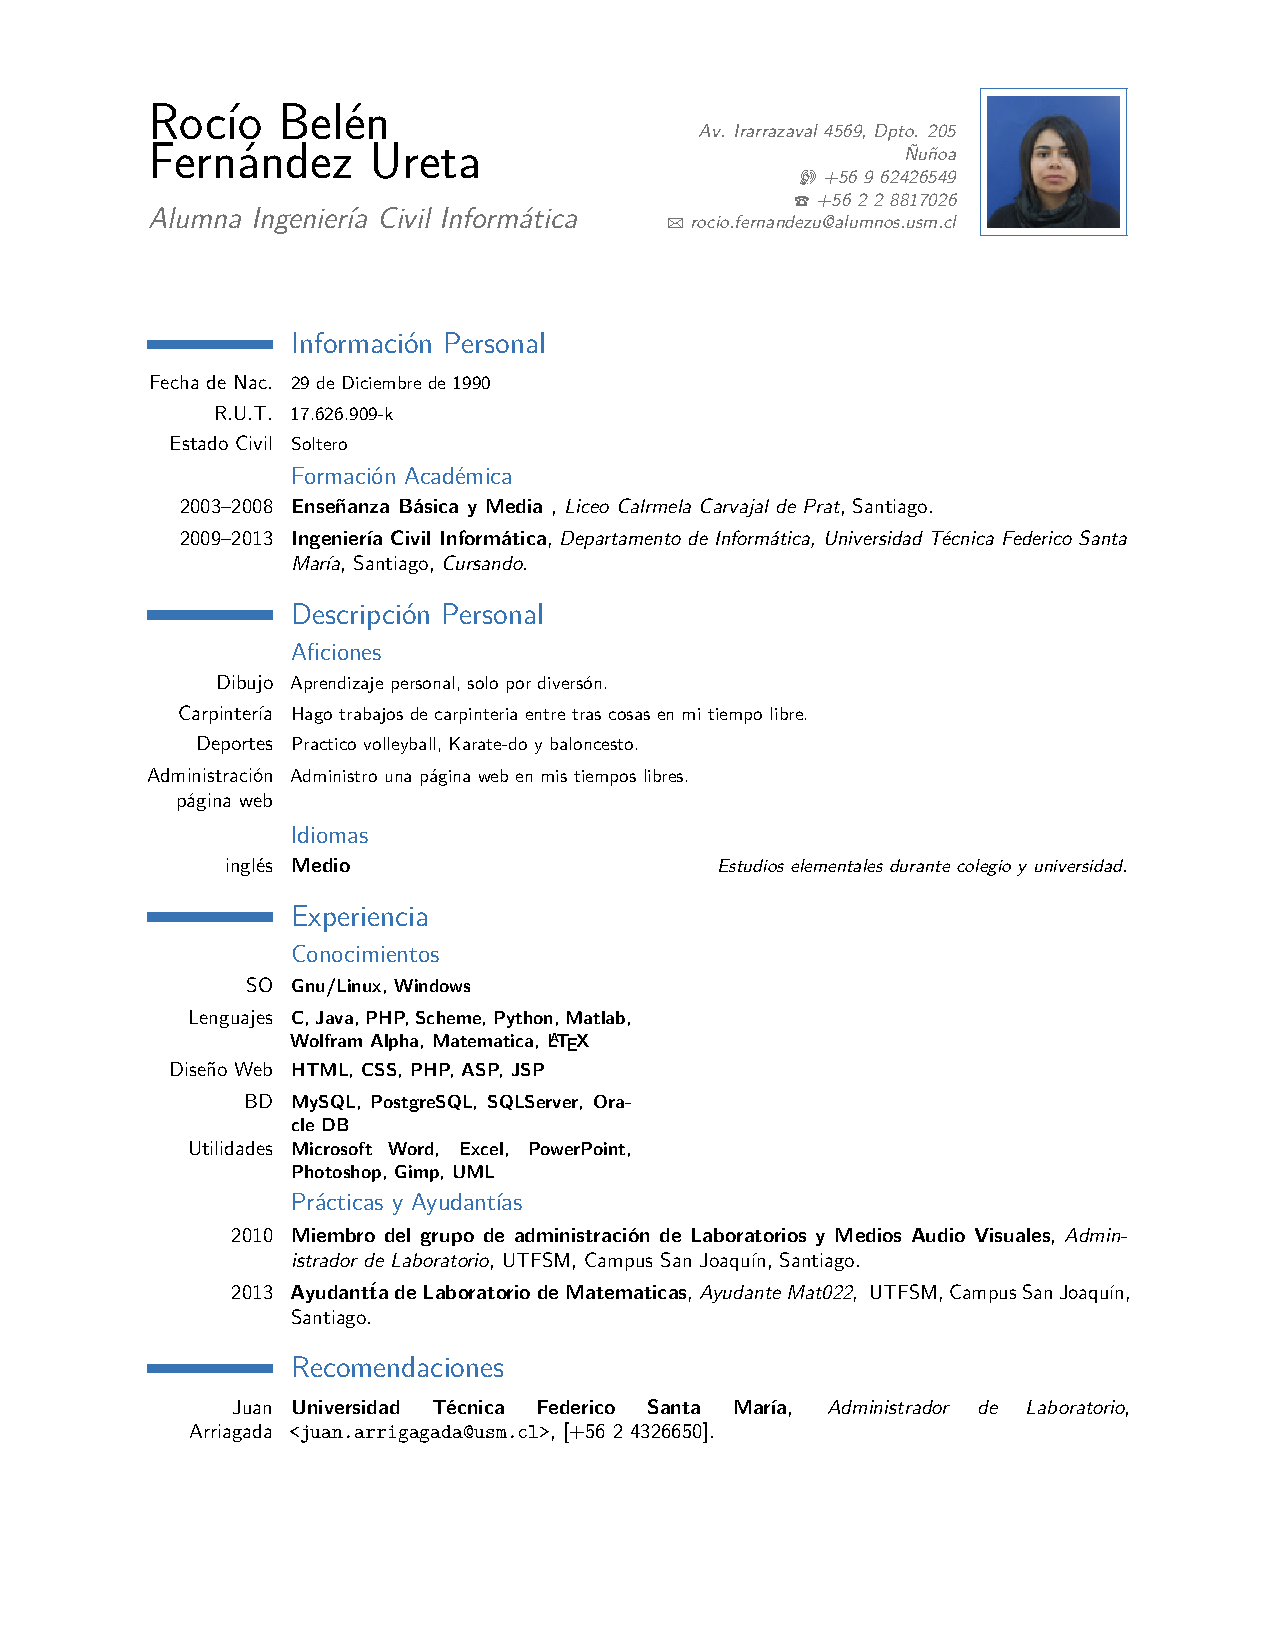
\includepdf[pages={1}]{../CV/cv-neko.pdf}
%\newpage
%\chapter*{Anexo III - Otros} %Otros


\end{document}
